\documentclass[1p]{elsarticle_modified}
%\bibliographystyle{elsarticle-num}

%\usepackage[colorlinks]{hyperref}
%\usepackage{abbrmath_seonhwa} %\Abb, \Ascr, \Acal ,\Abf, \Afrak
\usepackage{amsfonts}
\usepackage{amssymb}
\usepackage{amsmath}
\usepackage{amsthm}
\usepackage{scalefnt}
\usepackage{amsbsy}
\usepackage{kotex}
\usepackage{caption}
\usepackage{subfig}
\usepackage{color}
\usepackage{graphicx}
\usepackage{xcolor} %% white, black, red, green, blue, cyan, magenta, yellow
\usepackage{float}
\usepackage{setspace}
\usepackage{hyperref}

\usepackage{tikz}
\usetikzlibrary{arrows}

\usepackage{multirow}
\usepackage{array} % fixed length table
\usepackage{hhline}

%%%%%%%%%%%%%%%%%%%%%
\makeatletter
\renewcommand*\env@matrix[1][\arraystretch]{%
	\edef\arraystretch{#1}%
	\hskip -\arraycolsep
	\let\@ifnextchar\new@ifnextchar
	\array{*\c@MaxMatrixCols c}}
\makeatother %https://tex.stackexchange.com/questions/14071/how-can-i-increase-the-line-spacing-in-a-matrix
%%%%%%%%%%%%%%%

\usepackage[normalem]{ulem}

\newcommand{\msout}[1]{\ifmmode\text{\sout{\ensuremath{#1}}}\else\sout{#1}\fi}
%SOURCE: \msout is \stkout macro in https://tex.stackexchange.com/questions/20609/strikeout-in-math-mode

\newcommand{\cancel}[1]{
	\ifmmode
	{\color{red}\msout{#1}}
	\else
	{\color{red}\sout{#1}}
	\fi
}

\newcommand{\add}[1]{
	{\color{blue}\uwave{#1}}
}

\newcommand{\replace}[2]{
	\ifmmode
	{\color{red}\msout{#1}}{\color{blue}\uwave{#2}}
	\else
	{\color{red}\sout{#1}}{\color{blue}\uwave{#2}}
	\fi
}

\newcommand{\Sol}{\mathcal{S}} %segment
\newcommand{\D}{D} %diagram
\newcommand{\A}{\mathcal{A}} %arc


%%%%%%%%%%%%%%%%%%%%%%%%%%%%%5 test

\def\sl{\operatorname{\textup{SL}}(2,\Cbb)}
\def\psl{\operatorname{\textup{PSL}}(2,\Cbb)}
\def\quan{\mkern 1mu \triangleright \mkern 1mu}

\theoremstyle{definition}
\newtheorem{thm}{Theorem}[section]
\newtheorem{prop}[thm]{Proposition}
\newtheorem{lem}[thm]{Lemma}
\newtheorem{ques}[thm]{Question}
\newtheorem{cor}[thm]{Corollary}
\newtheorem{defn}[thm]{Definition}
\newtheorem{exam}[thm]{Example}
\newtheorem{rmk}[thm]{Remark}
\newtheorem{alg}[thm]{Algorithm}

\newcommand{\I}{\sqrt{-1}}
\begin{document}

%\begin{frontmatter}
%
%\title{Boundary parabolic representations of knots up to 8 crossings}
%
%%% Group authors per affiliation:
%\author{Yunhi Cho} 
%\address{Department of Mathematics, University of Seoul, Seoul, Korea}
%\ead{yhcho@uos.ac.kr}
%
%
%\author{Seonhwa Kim} %\fnref{s_kim}}
%\address{Center for Geometry and Physics, Institute for Basic Science, Pohang, 37673, Korea}
%\ead{ryeona17@ibs.re.kr}
%
%\author{Hyuk Kim}
%\address{Department of Mathematical Sciences, Seoul National University, Seoul 08826, Korea}
%\ead{hyukkim@snu.ac.kr}
%
%\author{Seokbeom Yoon}
%\address{Department of Mathematical Sciences, Seoul National University, Seoul, 08826,  Korea}
%\ead{sbyoon15@snu.ac.kr}
%
%\begin{abstract}
%We find all boundary parabolic representation of knots up to 8 crossings.
%
%\end{abstract}
%\begin{keyword}
%    \MSC[2010] 57M25 
%\end{keyword}
%
%\end{frontmatter}

%\linenumbers
%\tableofcontents
%
\newcommand\colored[1]{\textcolor{white}{\rule[-0.35ex]{0.8em}{1.4ex}}\kern-0.8em\color{red} #1}%
%\newcommand\colored[1]{\textcolor{white}{ #1}\kern-2.17ex	\textcolor{white}{ #1}\kern-1.81ex	\textcolor{white}{ #1}\kern-2.15ex\color{red}#1	}

{\Large $\underline{12n_{0836}~(K12n_{0836})}$}

\setlength{\tabcolsep}{10pt}
\renewcommand{\arraystretch}{1.6}
\vspace{1cm}\begin{tabular}{m{100pt}>{\centering\arraybackslash}m{274pt}}
\multirow{5}{120pt}{
	\centering
	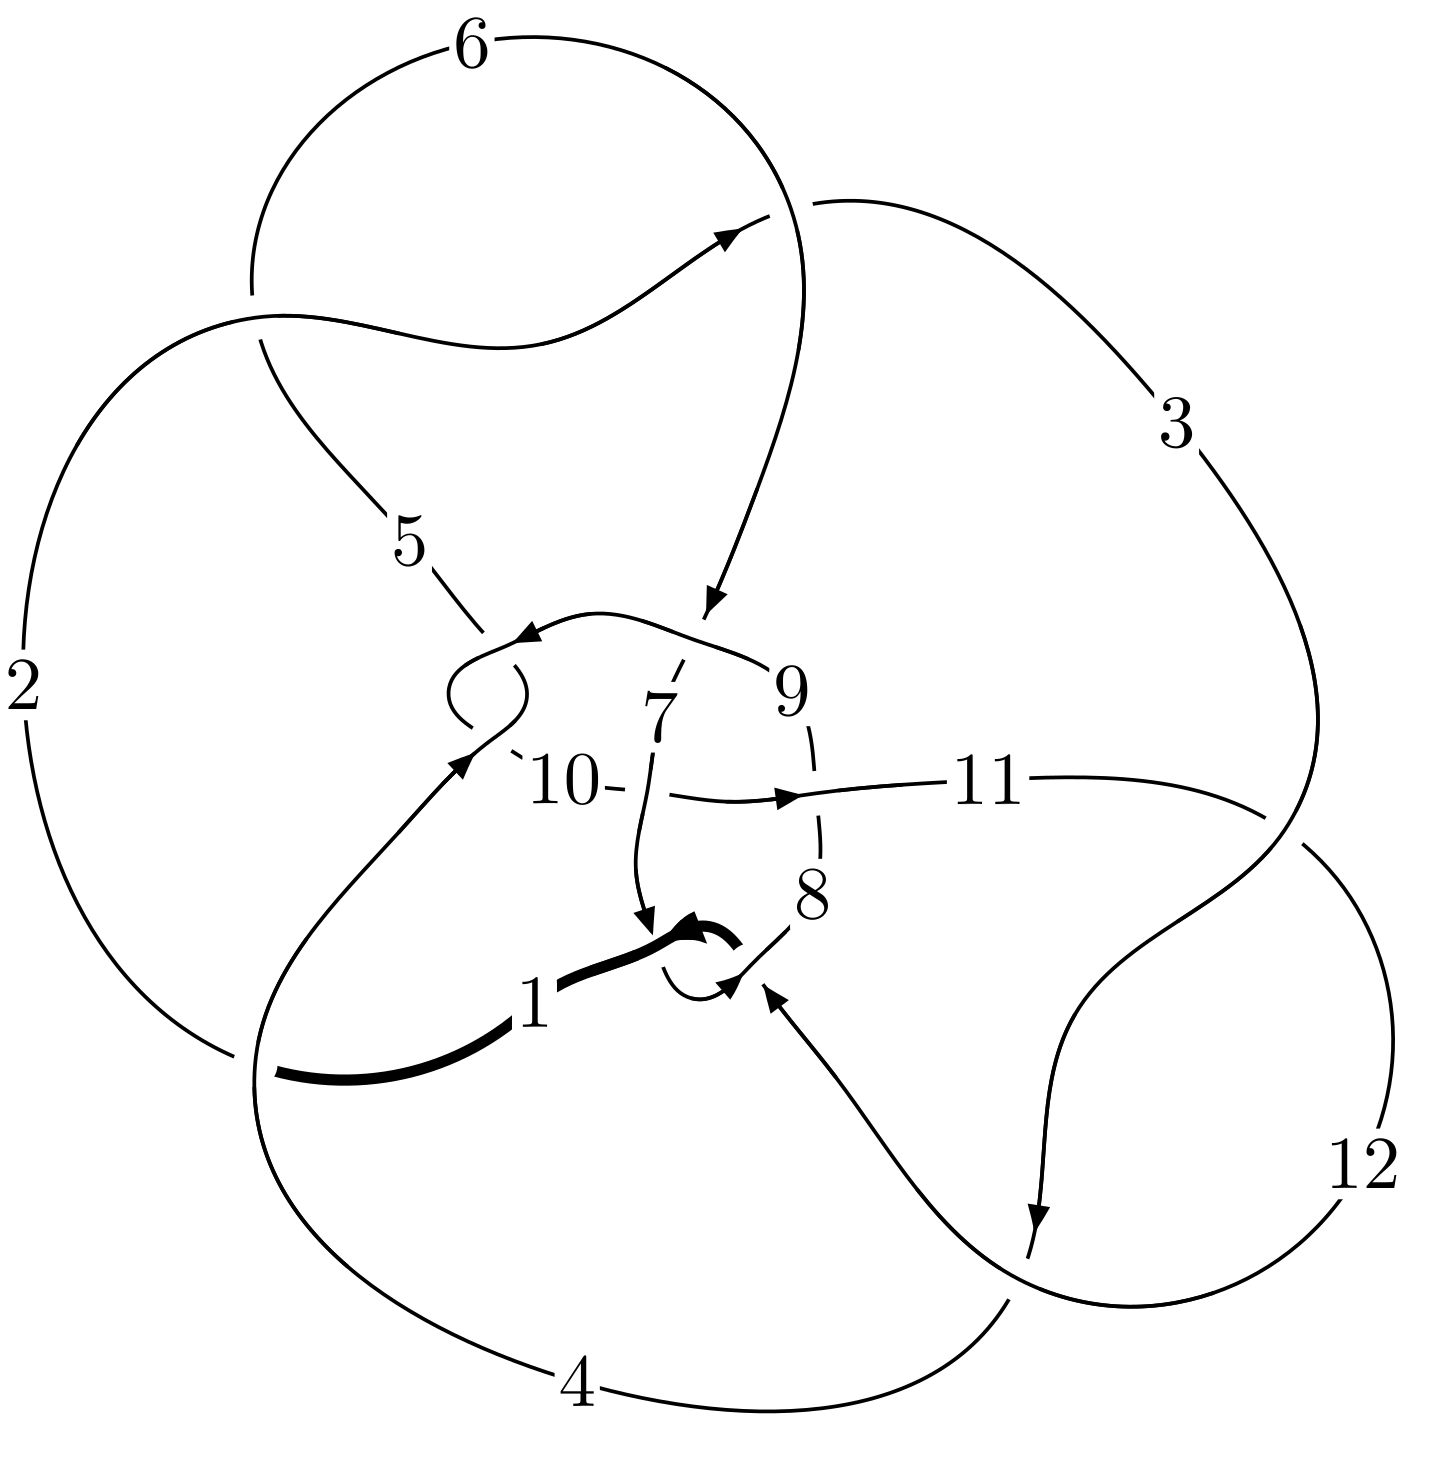
\includegraphics[width=112pt]{../../../GIT/diagram.site/Diagrams/png/2925_12n_0836.png}\\
\ \ \ A knot diagram\footnotemark}&
\allowdisplaybreaks
\textbf{Linearized knot diagam} \\
\cline{2-2}
 &
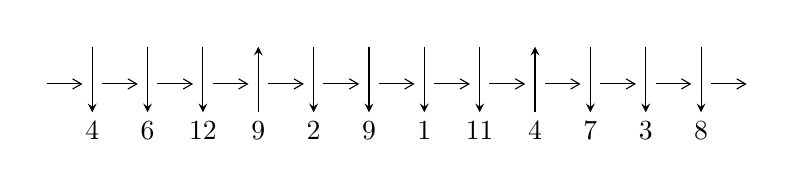
\begin{tikzpicture}[x=20pt, y=17pt]
	% nodes
	\node (C0) at (0, 0) {};
	\node (C1) at (1, 0) {};
	\node (C1U) at (1, +1) {};
	\node (C1D) at (1, -1) {4};

	\node (C2) at (2, 0) {};
	\node (C2U) at (2, +1) {};
	\node (C2D) at (2, -1) {6};

	\node (C3) at (3, 0) {};
	\node (C3U) at (3, +1) {};
	\node (C3D) at (3, -1) {12};

	\node (C4) at (4, 0) {};
	\node (C4U) at (4, +1) {};
	\node (C4D) at (4, -1) {9};

	\node (C5) at (5, 0) {};
	\node (C5U) at (5, +1) {};
	\node (C5D) at (5, -1) {2};

	\node (C6) at (6, 0) {};
	\node (C6U) at (6, +1) {};
	\node (C6D) at (6, -1) {9};

	\node (C7) at (7, 0) {};
	\node (C7U) at (7, +1) {};
	\node (C7D) at (7, -1) {1};

	\node (C8) at (8, 0) {};
	\node (C8U) at (8, +1) {};
	\node (C8D) at (8, -1) {11};

	\node (C9) at (9, 0) {};
	\node (C9U) at (9, +1) {};
	\node (C9D) at (9, -1) {4};

	\node (C10) at (10, 0) {};
	\node (C10U) at (10, +1) {};
	\node (C10D) at (10, -1) {7};

	\node (C11) at (11, 0) {};
	\node (C11U) at (11, +1) {};
	\node (C11D) at (11, -1) {3};

	\node (C12) at (12, 0) {};
	\node (C12U) at (12, +1) {};
	\node (C12D) at (12, -1) {8};
	\node (C13) at (13, 0) {};

	% arrows
	\draw[->,>={angle 60}]
	(C0) edge (C1) (C1) edge (C2) (C2) edge (C3) (C3) edge (C4) (C4) edge (C5) (C5) edge (C6) (C6) edge (C7) (C7) edge (C8) (C8) edge (C9) (C9) edge (C10) (C10) edge (C11) (C11) edge (C12) (C12) edge (C13) ;	\draw[->,>=stealth]
	(C1U) edge (C1D) (C2U) edge (C2D) (C3U) edge (C3D) (C4D) edge (C4U) (C5U) edge (C5D) (C6U) edge (C6D) (C7U) edge (C7D) (C8U) edge (C8D) (C9D) edge (C9U) (C10U) edge (C10D) (C11U) edge (C11D) (C12U) edge (C12D) ;
	\end{tikzpicture} \\
\hhline{~~} \\& 
\textbf{Solving Sequence} \\ \cline{2-2} 
 &
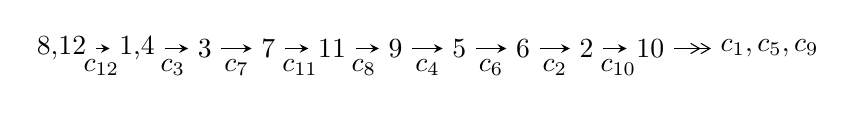
\begin{tikzpicture}[x=23pt, y=7pt]
	% node
	\node (A0) at (-1/8, 0) {8,12};
	\node (A1) at (17/16, 0) {1,4};
	\node (A2) at (17/8, 0) {3};
	\node (A3) at (25/8, 0) {7};
	\node (A4) at (33/8, 0) {11};
	\node (A5) at (41/8, 0) {9};
	\node (A6) at (49/8, 0) {5};
	\node (A7) at (57/8, 0) {6};
	\node (A8) at (65/8, 0) {2};
	\node (A9) at (73/8, 0) {10};
	\node (C1) at (1/2, -1) {$c_{12}$};
	\node (C2) at (13/8, -1) {$c_{3}$};
	\node (C3) at (21/8, -1) {$c_{7}$};
	\node (C4) at (29/8, -1) {$c_{11}$};
	\node (C5) at (37/8, -1) {$c_{8}$};
	\node (C6) at (45/8, -1) {$c_{4}$};
	\node (C7) at (53/8, -1) {$c_{6}$};
	\node (C8) at (61/8, -1) {$c_{2}$};
	\node (C9) at (69/8, -1) {$c_{10}$};
	\node (A10) at (11, 0) {$c_{1},c_{5},c_{9}$};

	% edge
	\draw[->,>=stealth]	
	(A0) edge (A1) (A1) edge (A2) (A2) edge (A3) (A3) edge (A4) (A4) edge (A5) (A5) edge (A6) (A6) edge (A7) (A7) edge (A8) (A8) edge (A9) ;
	\draw[->>,>={angle 60}]	
	(A9) edge (A10);
\end{tikzpicture} \\ 

\end{tabular} \\

\footnotetext{
The image of knot diagram is generated by the software ``\textbf{Draw programme}" developed by Andrew Bartholomew(\url{http://www.layer8.co.uk/maths/draw/index.htm\#Running-draw}), where we modified some parts for our purpose(\url{https://github.com/CATsTAILs/LinksPainter}).
}\phantom \\ \newline 
\centering \textbf{Ideals for irreducible components\footnotemark of $X_{\text{par}}$} 
 
\begin{align*}
I^u_{1}&=\langle 
-2.01141\times10^{178} u^{79}-1.53427\times10^{179} u^{78}+\cdots+8.20723\times10^{178} b+1.11833\times10^{181},\\
\phantom{I^u_{1}}&\phantom{= \langle  }-8.82110\times10^{179} u^{79}-1.86815\times10^{180} u^{78}+\cdots+4.33810\times10^{179} a-1.20564\times10^{182},\\
\phantom{I^u_{1}}&\phantom{= \langle  }u^{80}+3 u^{79}+\cdots-692 u-148\rangle \\
I^u_{2}&=\langle 
-419743649 u^{22}+600334478 u^{21}+\cdots+939590426 b+1322008284,\\
\phantom{I^u_{2}}&\phantom{= \langle  }544158953 u^{22}-1664036159 u^{21}+\cdots+1879180852 a-3189273440,\;u^{23}- u^{22}+\cdots+8 u+4\rangle \\
I^u_{3}&=\langle 
b+1,\;a+1,\;u-1\rangle \\
\\
\end{align*}
\raggedright * 3 irreducible components of $\dim_{\mathbb{C}}=0$, with total 104 representations.\\
\footnotetext{All coefficients of polynomials are rational numbers. But the coefficients are sometimes approximated in decimal forms when there is not enough margin.}
\newpage
\renewcommand{\arraystretch}{1}
\centering \section*{I. $I^u_{1}= \langle -2.01\times10^{178} u^{79}-1.53\times10^{179} u^{78}+\cdots+8.21\times10^{178} b+1.12\times10^{181},\;-8.82\times10^{179} u^{79}-1.87\times10^{180} u^{78}+\cdots+4.34\times10^{179} a-1.21\times10^{182},\;u^{80}+3 u^{79}+\cdots-692 u-148 \rangle$}
\flushleft \textbf{(i) Arc colorings}\\
\begin{tabular}{m{7pt} m{180pt} m{7pt} m{180pt} }
\flushright $a_{8}=$&$\begin{pmatrix}0\\u\end{pmatrix}$ \\
\flushright $a_{12}=$&$\begin{pmatrix}1\\0\end{pmatrix}$ \\
\flushright $a_{1}=$&$\begin{pmatrix}1\\u^2\end{pmatrix}$ \\
\flushright $a_{4}=$&$\begin{pmatrix}2.03340 u^{79}+4.30637 u^{78}+\cdots+1080.35 u+277.919\\0.245078 u^{79}+1.86942 u^{78}+\cdots-692.484 u-136.261\end{pmatrix}$ \\
\flushright $a_{3}=$&$\begin{pmatrix}2.27848 u^{79}+6.17578 u^{78}+\cdots+387.869 u+141.658\\0.245078 u^{79}+1.86942 u^{78}+\cdots-692.484 u-136.261\end{pmatrix}$ \\
\flushright $a_{7}=$&$\begin{pmatrix}u\\u^3+u\end{pmatrix}$ \\
\flushright $a_{11}=$&$\begin{pmatrix}-0.261711 u^{79}-0.131889 u^{78}+\cdots-408.221 u-92.9224\\-0.447967 u^{79}-2.59603 u^{78}+\cdots+801.323 u+153.979\end{pmatrix}$ \\
\flushright $a_{9}=$&$\begin{pmatrix}0.937727 u^{79}+2.63334 u^{78}+\cdots+85.3324 u+42.4994\\-0.149265 u^{79}-0.548385 u^{78}+\cdots+52.3634 u+9.08703\end{pmatrix}$ \\
\flushright $a_{5}=$&$\begin{pmatrix}10.1203 u^{79}+29.8622 u^{78}+\cdots+201.630 u+315.128\\0.0269954 u^{79}+2.97414 u^{78}+\cdots-1810.20 u-372.735\end{pmatrix}$ \\
\flushright $a_{6}=$&$\begin{pmatrix}-2.15415 u^{79}-4.52646 u^{78}+\cdots-1317.07 u-333.037\\0.0899931 u^{79}-0.186489 u^{78}+\cdots+277.477 u+59.4733\end{pmatrix}$ \\
\flushright $a_{2}=$&$\begin{pmatrix}-0.980754 u^{79}-4.52806 u^{78}+\cdots+1187.82 u+218.399\\0.419539 u^{79}+0.305039 u^{78}+\cdots+544.761 u+128.017\end{pmatrix}$ \\
\flushright $a_{10}=$&$\begin{pmatrix}0.135237 u^{79}+2.49572 u^{78}+\cdots-1315.46 u-271.021\\-0.303249 u^{79}-2.42157 u^{78}+\cdots+947.070 u+188.521\end{pmatrix}$\\&\end{tabular}
\flushleft \textbf{(ii) Obstruction class $= -1$}\\~\\
\flushleft \textbf{(iii) Cusp Shapes $= 4.02688 u^{79}+13.5179 u^{78}+\cdots-913.018 u-91.2459$}\\~\\
\newpage\renewcommand{\arraystretch}{1}
\flushleft \textbf{(iv) u-Polynomials at the component}\newline \\
\begin{tabular}{m{50pt}|m{274pt}}
Crossings & \hspace{64pt}u-Polynomials at each crossing \\
\hline $$\begin{aligned}c_{1}\end{aligned}$$&$\begin{aligned}
&u^{80}+u^{79}+\cdots+121816053 u+10935405
\end{aligned}$\\
\hline $$\begin{aligned}c_{2},c_{5}\end{aligned}$$&$\begin{aligned}
&u^{80}+5 u^{79}+\cdots-9 u+1
\end{aligned}$\\
\hline $$\begin{aligned}c_{3},c_{11}\end{aligned}$$&$\begin{aligned}
&u^{80}+2 u^{79}+\cdots-488 u-91
\end{aligned}$\\
\hline $$\begin{aligned}c_{4},c_{9}\end{aligned}$$&$\begin{aligned}
&u^{80}-4 u^{79}+\cdots+22580 u+3676
\end{aligned}$\\
\hline $$\begin{aligned}c_{6}\end{aligned}$$&$\begin{aligned}
&u^{80}-8 u^{79}+\cdots+11892000 u+986616
\end{aligned}$\\
\hline $$\begin{aligned}c_{7},c_{12}\end{aligned}$$&$\begin{aligned}
&u^{80}+3 u^{79}+\cdots-692 u-148
\end{aligned}$\\
\hline $$\begin{aligned}c_{8}\end{aligned}$$&$\begin{aligned}
&u^{80}-11 u^{79}+\cdots+258 u-11
\end{aligned}$\\
\hline $$\begin{aligned}c_{10}\end{aligned}$$&$\begin{aligned}
&u^{80}-4 u^{79}+\cdots+9331040 u+665887
\end{aligned}$\\
\hline
\end{tabular}\\~\\
\newpage\renewcommand{\arraystretch}{1}
\flushleft \textbf{(v) Riley Polynomials at the component}\newline \\
\begin{tabular}{m{50pt}|m{274pt}}
Crossings & \hspace{64pt}Riley Polynomials at each crossing \\
\hline $$\begin{aligned}c_{1}\end{aligned}$$&$\begin{aligned}
&y^{80}+59 y^{79}+\cdots+3158025656114421 y+119583082514025
\end{aligned}$\\
\hline $$\begin{aligned}c_{2},c_{5}\end{aligned}$$&$\begin{aligned}
&y^{80}-21 y^{79}+\cdots-63 y+1
\end{aligned}$\\
\hline $$\begin{aligned}c_{3},c_{11}\end{aligned}$$&$\begin{aligned}
&y^{80}-46 y^{79}+\cdots-130946 y+8281
\end{aligned}$\\
\hline $$\begin{aligned}c_{4},c_{9}\end{aligned}$$&$\begin{aligned}
&y^{80}-80 y^{79}+\cdots-1476835552 y+13512976
\end{aligned}$\\
\hline $$\begin{aligned}c_{6}\end{aligned}$$&$\begin{aligned}
&y^{80}+58 y^{79}+\cdots-53110665152640 y+973411131456
\end{aligned}$\\
\hline $$\begin{aligned}c_{7},c_{12}\end{aligned}$$&$\begin{aligned}
&y^{80}+57 y^{79}+\cdots+262912 y+21904
\end{aligned}$\\
\hline $$\begin{aligned}c_{8}\end{aligned}$$&$\begin{aligned}
&y^{80}+3 y^{79}+\cdots-8880 y+121
\end{aligned}$\\
\hline $$\begin{aligned}c_{10}\end{aligned}$$&$\begin{aligned}
&y^{80}+46 y^{79}+\cdots-72020481186584 y+443405496769
\end{aligned}$\\
\hline
\end{tabular}\\~\\
\newpage\flushleft \textbf{(vi) Complex Volumes and Cusp Shapes}
$$\begin{array}{c|c|c}  
\text{Solutions to }I^u_{1}& \I (\text{vol} + \sqrt{-1}CS) & \text{Cusp shape}\\
 \hline 
\begin{aligned}
u &= \phantom{-}0.046801 + 1.002510 I \\
a &= \phantom{-}0.98336 + 1.75820 I \\
b &= -0.573536 - 0.982987 I\end{aligned}
 & -0.176447 - 0.015979 I & \phantom{-0.000000 } 0 \\ \hline\begin{aligned}
u &= \phantom{-}0.046801 - 1.002510 I \\
a &= \phantom{-}0.98336 - 1.75820 I \\
b &= -0.573536 + 0.982987 I\end{aligned}
 & -0.176447 + 0.015979 I & \phantom{-0.000000 } 0 \\ \hline\begin{aligned}
u &= \phantom{-}0.822278 + 0.475094 I \\
a &= \phantom{-}0.732335 - 0.357721 I \\
b &= \phantom{-}0.957847 - 0.349248 I\end{aligned}
 & -2.53039 + 3.09745 I & \phantom{-0.000000 } 0 \\ \hline\begin{aligned}
u &= \phantom{-}0.822278 - 0.475094 I \\
a &= \phantom{-}0.732335 + 0.357721 I \\
b &= \phantom{-}0.957847 + 0.349248 I\end{aligned}
 & -2.53039 - 3.09745 I & \phantom{-0.000000 } 0 \\ \hline\begin{aligned}
u &= \phantom{-}0.091622 + 1.055600 I \\
a &= \phantom{-}0.24639 + 2.94466 I \\
b &= \phantom{-}0.822173 - 0.286394 I\end{aligned}
 & \phantom{-}6.28320 - 3.62041 I & \phantom{-0.000000 } 0 \\ \hline\begin{aligned}
u &= \phantom{-}0.091622 - 1.055600 I \\
a &= \phantom{-}0.24639 - 2.94466 I \\
b &= \phantom{-}0.822173 + 0.286394 I\end{aligned}
 & \phantom{-}6.28320 + 3.62041 I & \phantom{-0.000000 } 0 \\ \hline\begin{aligned}
u &= \phantom{-}0.279779 + 1.030260 I \\
a &= -0.01582 + 2.20267 I \\
b &= -1.160090 - 0.565372 I\end{aligned}
 & -2.43822 - 5.49446 I & \phantom{-0.000000 } 0 \\ \hline\begin{aligned}
u &= \phantom{-}0.279779 - 1.030260 I \\
a &= -0.01582 - 2.20267 I \\
b &= -1.160090 + 0.565372 I\end{aligned}
 & -2.43822 + 5.49446 I & \phantom{-0.000000 } 0 \\ \hline\begin{aligned}
u &= -0.255565 + 0.885376 I \\
a &= \phantom{-}1.192220 - 0.536184 I \\
b &= -1.74649 + 0.21439 I\end{aligned}
 & \phantom{-}1.24011 + 5.04477 I & \phantom{-0.000000 } 0 \\ \hline\begin{aligned}
u &= -0.255565 - 0.885376 I \\
a &= \phantom{-}1.192220 + 0.536184 I \\
b &= -1.74649 - 0.21439 I\end{aligned}
 & \phantom{-}1.24011 - 5.04477 I & \phantom{-0.000000 } 0\\
 \hline 
 \end{array}$$\newpage$$\begin{array}{c|c|c}  
\text{Solutions to }I^u_{1}& \I (\text{vol} + \sqrt{-1}CS) & \text{Cusp shape}\\
 \hline 
\begin{aligned}
u &= \phantom{-}0.105049 + 1.089820 I \\
a &= \phantom{-}0.41716 - 2.72556 I \\
b &= -0.757713 + 0.316934 I\end{aligned}
 & \phantom{-}6.31846 + 2.49469 I & \phantom{-0.000000 } 0 \\ \hline\begin{aligned}
u &= \phantom{-}0.105049 - 1.089820 I \\
a &= \phantom{-}0.41716 + 2.72556 I \\
b &= -0.757713 - 0.316934 I\end{aligned}
 & \phantom{-}6.31846 - 2.49469 I & \phantom{-0.000000 } 0 \\ \hline\begin{aligned}
u &= \phantom{-}0.081923 + 1.111640 I \\
a &= -0.93761 - 1.73433 I \\
b &= \phantom{-}1.45583 + 1.02764 I\end{aligned}
 & \phantom{-}3.16613 - 5.16687 I & \phantom{-0.000000 } 0 \\ \hline\begin{aligned}
u &= \phantom{-}0.081923 - 1.111640 I \\
a &= -0.93761 + 1.73433 I \\
b &= \phantom{-}1.45583 - 1.02764 I\end{aligned}
 & \phantom{-}3.16613 + 5.16687 I & \phantom{-0.000000 } 0 \\ \hline\begin{aligned}
u &= \phantom{-}0.306815 + 0.809611 I \\
a &= -0.59543 + 1.62433 I \\
b &= \phantom{-}0.680031 - 1.128500 I\end{aligned}
 & -1.13568 - 1.39327 I & \phantom{-0.000000 -}0. + 6.02870 I \\ \hline\begin{aligned}
u &= \phantom{-}0.306815 - 0.809611 I \\
a &= -0.59543 - 1.62433 I \\
b &= \phantom{-}0.680031 + 1.128500 I\end{aligned}
 & -1.13568 + 1.39327 I & \phantom{-0.000000 } 0. - 6.02870 I \\ \hline\begin{aligned}
u &= \phantom{-}0.850618 + 0.141619 I \\
a &= -0.603834 - 0.644927 I \\
b &= -0.082168 + 0.834234 I\end{aligned}
 & \phantom{-}4.31948 - 6.02401 I & -8.00000 + 4.76540 I \\ \hline\begin{aligned}
u &= \phantom{-}0.850618 - 0.141619 I \\
a &= -0.603834 + 0.644927 I \\
b &= -0.082168 - 0.834234 I\end{aligned}
 & \phantom{-}4.31948 + 6.02401 I & -8.00000 - 4.76540 I \\ \hline\begin{aligned}
u &= -0.393225 + 1.082950 I \\
a &= \phantom{-}0.149783 - 1.328200 I \\
b &= -1.077820 + 0.560087 I\end{aligned}
 & \phantom{-}1.63816 + 3.25672 I & \phantom{-0.000000 } 0 \\ \hline\begin{aligned}
u &= -0.393225 - 1.082950 I \\
a &= \phantom{-}0.149783 + 1.328200 I \\
b &= -1.077820 - 0.560087 I\end{aligned}
 & \phantom{-}1.63816 - 3.25672 I & \phantom{-0.000000 } 0\\
 \hline 
 \end{array}$$\newpage$$\begin{array}{c|c|c}  
\text{Solutions to }I^u_{1}& \I (\text{vol} + \sqrt{-1}CS) & \text{Cusp shape}\\
 \hline 
\begin{aligned}
u &= \phantom{-}0.010130 + 0.814360 I \\
a &= \phantom{-}0.298622 + 1.013230 I \\
b &= \phantom{-}1.011000 - 0.400621 I\end{aligned}
 & -0.745254 - 0.723458 I & -9.33301 + 2.88959 I \\ \hline\begin{aligned}
u &= \phantom{-}0.010130 - 0.814360 I \\
a &= \phantom{-}0.298622 - 1.013230 I \\
b &= \phantom{-}1.011000 + 0.400621 I\end{aligned}
 & -0.745254 + 0.723458 I & -9.33301 - 2.88959 I \\ \hline\begin{aligned}
u &= \phantom{-}0.765524 + 0.242345 I \\
a &= \phantom{-}0.829280 + 0.521861 I \\
b &= \phantom{-}0.120637 - 0.711335 I\end{aligned}
 & \phantom{-}5.10844 + 0.82388 I & -5.14125 - 0.25076 I \\ \hline\begin{aligned}
u &= \phantom{-}0.765524 - 0.242345 I \\
a &= \phantom{-}0.829280 - 0.521861 I \\
b &= \phantom{-}0.120637 + 0.711335 I\end{aligned}
 & \phantom{-}5.10844 - 0.82388 I & -5.14125 + 0.25076 I \\ \hline\begin{aligned}
u &= \phantom{-}0.540193 + 0.561625 I \\
a &= \phantom{-}0.470096 - 0.502904 I \\
b &= \phantom{-}1.121930 - 0.386740 I\end{aligned}
 & -3.79395 + 2.22531 I & -15.1723 + 3.2449 I \\ \hline\begin{aligned}
u &= \phantom{-}0.540193 - 0.561625 I \\
a &= \phantom{-}0.470096 + 0.502904 I \\
b &= \phantom{-}1.121930 + 0.386740 I\end{aligned}
 & -3.79395 - 2.22531 I & -15.1723 - 3.2449 I \\ \hline\begin{aligned}
u &= \phantom{-}0.491737 + 1.117400 I \\
a &= -0.54139 + 1.52861 I \\
b &= -1.131240 - 0.476408 I\end{aligned}
 & -0.42712 - 8.03019 I & \phantom{-0.000000 } 0 \\ \hline\begin{aligned}
u &= \phantom{-}0.491737 - 1.117400 I \\
a &= -0.54139 - 1.52861 I \\
b &= -1.131240 + 0.476408 I\end{aligned}
 & -0.42712 + 8.03019 I & \phantom{-0.000000 } 0 \\ \hline\begin{aligned}
u &= -1.224740 + 0.000179 I \\
a &= \phantom{-}0.246321 + 0.350162 I \\
b &= \phantom{-}1.144690 - 0.486456 I\end{aligned}
 & \phantom{-}2.22985 + 3.62423 I & \phantom{-0.000000 } 0 \\ \hline\begin{aligned}
u &= -1.224740 - 0.000179 I \\
a &= \phantom{-}0.246321 - 0.350162 I \\
b &= \phantom{-}1.144690 + 0.486456 I\end{aligned}
 & \phantom{-}2.22985 - 3.62423 I & \phantom{-0.000000 } 0\\
 \hline 
 \end{array}$$\newpage$$\begin{array}{c|c|c}  
\text{Solutions to }I^u_{1}& \I (\text{vol} + \sqrt{-1}CS) & \text{Cusp shape}\\
 \hline 
\begin{aligned}
u &= -0.306758 + 1.193560 I \\
a &= \phantom{-}0.435738 + 0.477747 I \\
b &= -0.212987 - 0.588066 I\end{aligned}
 & \phantom{-}2.19021 + 3.79104 I & \phantom{-0.000000 } 0 \\ \hline\begin{aligned}
u &= -0.306758 - 1.193560 I \\
a &= \phantom{-}0.435738 - 0.477747 I \\
b &= -0.212987 + 0.588066 I\end{aligned}
 & \phantom{-}2.19021 - 3.79104 I & \phantom{-0.000000 } 0 \\ \hline\begin{aligned}
u &= -1.235680 + 0.050440 I \\
a &= -0.272628 - 0.464013 I \\
b &= -1.206980 + 0.505362 I\end{aligned}
 & \phantom{-}1.01408 + 10.86440 I & \phantom{-0.000000 } 0 \\ \hline\begin{aligned}
u &= -1.235680 - 0.050440 I \\
a &= -0.272628 + 0.464013 I \\
b &= -1.206980 - 0.505362 I\end{aligned}
 & \phantom{-}1.01408 - 10.86440 I & \phantom{-0.000000 } 0 \\ \hline\begin{aligned}
u &= \phantom{-}1.23866\phantom{ +0.000000I} \\
a &= -0.818757\phantom{ +0.000000I} \\
b &= -0.903518\phantom{ +0.000000I}\end{aligned}
 & -4.96766\phantom{ +0.000000I} & \phantom{-0.000000 } 0 \\ \hline\begin{aligned}
u &= \phantom{-}0.287804 + 1.205310 I \\
a &= -0.07226 - 1.48666 I \\
b &= \phantom{-}1.35004 + 0.46853 I\end{aligned}
 & -1.05609 - 7.02185 I & \phantom{-0.000000 } 0 \\ \hline\begin{aligned}
u &= \phantom{-}0.287804 - 1.205310 I \\
a &= -0.07226 + 1.48666 I \\
b &= \phantom{-}1.35004 - 0.46853 I\end{aligned}
 & -1.05609 + 7.02185 I & \phantom{-0.000000 } 0 \\ \hline\begin{aligned}
u &= -0.037339 + 1.249590 I \\
a &= \phantom{-}0.008119 - 1.158290 I \\
b &= -0.278270 + 0.933238 I\end{aligned}
 & \phantom{-}3.92396 + 2.10466 I & \phantom{-0.000000 } 0 \\ \hline\begin{aligned}
u &= -0.037339 - 1.249590 I \\
a &= \phantom{-}0.008119 + 1.158290 I \\
b &= -0.278270 - 0.933238 I\end{aligned}
 & \phantom{-}3.92396 - 2.10466 I & \phantom{-0.000000 } 0 \\ \hline\begin{aligned}
u &= -0.717179 + 0.064230 I \\
a &= \phantom{-}0.389771 - 0.052663 I \\
b &= \phantom{-}0.500055 - 0.258503 I\end{aligned}
 & -1.354540 - 0.079357 I & -5.49507 - 1.06068 I\\
 \hline 
 \end{array}$$\newpage$$\begin{array}{c|c|c}  
\text{Solutions to }I^u_{1}& \I (\text{vol} + \sqrt{-1}CS) & \text{Cusp shape}\\
 \hline 
\begin{aligned}
u &= -0.717179 - 0.064230 I \\
a &= \phantom{-}0.389771 + 0.052663 I \\
b &= \phantom{-}0.500055 + 0.258503 I\end{aligned}
 & -1.354540 + 0.079357 I & -5.49507 + 1.06068 I \\ \hline\begin{aligned}
u &= -0.548102 + 0.419477 I \\
a &= -0.34153 + 1.63307 I \\
b &= \phantom{-}1.310210 - 0.401158 I\end{aligned}
 & \phantom{-}0.18162 - 1.54489 I & -11.98300 + 1.73737 I \\ \hline\begin{aligned}
u &= -0.548102 - 0.419477 I \\
a &= -0.34153 - 1.63307 I \\
b &= \phantom{-}1.310210 + 0.401158 I\end{aligned}
 & \phantom{-}0.18162 + 1.54489 I & -11.98300 - 1.73737 I \\ \hline\begin{aligned}
u &= -0.128278 + 1.308850 I \\
a &= \phantom{-}0.334243 - 1.179070 I \\
b &= -0.661054 + 0.678245 I\end{aligned}
 & \phantom{-}3.31548 + 2.64034 I & \phantom{-0.000000 } 0 \\ \hline\begin{aligned}
u &= -0.128278 - 1.308850 I \\
a &= \phantom{-}0.334243 + 1.179070 I \\
b &= -0.661054 - 0.678245 I\end{aligned}
 & \phantom{-}3.31548 - 2.64034 I & \phantom{-0.000000 } 0 \\ \hline\begin{aligned}
u &= \phantom{-}0.418017 + 1.260320 I \\
a &= \phantom{-}0.254230 - 1.347270 I \\
b &= \phantom{-}1.153920 + 0.328092 I\end{aligned}
 & -1.18466 - 4.83399 I & \phantom{-0.000000 } 0 \\ \hline\begin{aligned}
u &= \phantom{-}0.418017 - 1.260320 I \\
a &= \phantom{-}0.254230 + 1.347270 I \\
b &= \phantom{-}1.153920 - 0.328092 I\end{aligned}
 & -1.18466 + 4.83399 I & \phantom{-0.000000 } 0 \\ \hline\begin{aligned}
u &= -0.148559 + 1.327950 I \\
a &= -1.80054 + 1.36603 I \\
b &= \phantom{-}0.897881 - 0.303281 I\end{aligned}
 & \phantom{-}6.00828 + 6.28936 I & \phantom{-0.000000 } 0 \\ \hline\begin{aligned}
u &= -0.148559 - 1.327950 I \\
a &= -1.80054 - 1.36603 I \\
b &= \phantom{-}0.897881 + 0.303281 I\end{aligned}
 & \phantom{-}6.00828 - 6.28936 I & \phantom{-0.000000 } 0 \\ \hline\begin{aligned}
u &= -1.276820 + 0.458507 I \\
a &= \phantom{-}0.0642039 + 0.1102510 I \\
b &= -1.137630 - 0.262063 I\end{aligned}
 & -6.57602 - 0.89051 I & \phantom{-0.000000 } 0\\
 \hline 
 \end{array}$$\newpage$$\begin{array}{c|c|c}  
\text{Solutions to }I^u_{1}& \I (\text{vol} + \sqrt{-1}CS) & \text{Cusp shape}\\
 \hline 
\begin{aligned}
u &= -1.276820 - 0.458507 I \\
a &= \phantom{-}0.0642039 - 0.1102510 I \\
b &= -1.137630 + 0.262063 I\end{aligned}
 & -6.57602 + 0.89051 I & \phantom{-0.000000 } 0 \\ \hline\begin{aligned}
u &= \phantom{-}0.375344 + 1.305330 I \\
a &= \phantom{-}0.45582 - 1.38696 I \\
b &= -0.316427 + 1.215260 I\end{aligned}
 & \phantom{-}9.73007 - 3.25378 I & \phantom{-0.000000 } 0 \\ \hline\begin{aligned}
u &= \phantom{-}0.375344 - 1.305330 I \\
a &= \phantom{-}0.45582 + 1.38696 I \\
b &= -0.316427 - 1.215260 I\end{aligned}
 & \phantom{-}9.73007 + 3.25378 I & \phantom{-0.000000 } 0 \\ \hline\begin{aligned}
u &= -0.156318 + 1.363940 I \\
a &= \phantom{-}1.34534 - 1.61897 I \\
b &= -0.905799 + 0.399198 I\end{aligned}
 & \phantom{-}5.74714 + 0.69667 I & \phantom{-0.000000 } 0 \\ \hline\begin{aligned}
u &= -0.156318 - 1.363940 I \\
a &= \phantom{-}1.34534 + 1.61897 I \\
b &= -0.905799 - 0.399198 I\end{aligned}
 & \phantom{-}5.74714 - 0.69667 I & \phantom{-0.000000 } 0 \\ \hline\begin{aligned}
u &= \phantom{-}0.419691 + 1.331690 I \\
a &= -0.51408 + 1.35772 I \\
b &= \phantom{-}0.280095 - 1.188640 I\end{aligned}
 & \phantom{-}8.83649 - 10.61630 I & \phantom{-0.000000 } 0 \\ \hline\begin{aligned}
u &= \phantom{-}0.419691 - 1.331690 I \\
a &= -0.51408 - 1.35772 I \\
b &= \phantom{-}0.280095 + 1.188640 I\end{aligned}
 & \phantom{-}8.83649 + 10.61630 I & \phantom{-0.000000 } 0 \\ \hline\begin{aligned}
u &= -0.127688 + 1.402740 I \\
a &= -1.017010 - 0.198866 I \\
b &= \phantom{-}0.712556 - 0.016753 I\end{aligned}
 & \phantom{-}1.28019 + 3.07152 I & \phantom{-0.000000 } 0 \\ \hline\begin{aligned}
u &= -0.127688 - 1.402740 I \\
a &= -1.017010 + 0.198866 I \\
b &= \phantom{-}0.712556 + 0.016753 I\end{aligned}
 & \phantom{-}1.28019 - 3.07152 I & \phantom{-0.000000 } 0 \\ \hline\begin{aligned}
u &= -0.69061 + 1.25085 I \\
a &= -0.287373 + 1.369720 I \\
b &= \phantom{-}1.233370 - 0.610545 I\end{aligned}
 & -3.79073 + 7.70099 I & \phantom{-0.000000 } 0\\
 \hline 
 \end{array}$$\newpage$$\begin{array}{c|c|c}  
\text{Solutions to }I^u_{1}& \I (\text{vol} + \sqrt{-1}CS) & \text{Cusp shape}\\
 \hline 
\begin{aligned}
u &= -0.69061 - 1.25085 I \\
a &= -0.287373 - 1.369720 I \\
b &= \phantom{-}1.233370 + 0.610545 I\end{aligned}
 & -3.79073 - 7.70099 I & \phantom{-0.000000 } 0 \\ \hline\begin{aligned}
u &= \phantom{-}0.509923 + 0.167049 I \\
a &= -1.18077 + 1.18242 I \\
b &= -1.183380 + 0.287450 I\end{aligned}
 & -4.27418 + 3.88356 I & -16.0855 - 8.1336 I \\ \hline\begin{aligned}
u &= \phantom{-}0.509923 - 0.167049 I \\
a &= -1.18077 - 1.18242 I \\
b &= -1.183380 - 0.287450 I\end{aligned}
 & -4.27418 - 3.88356 I & -16.0855 + 8.1336 I \\ \hline\begin{aligned}
u &= \phantom{-}0.73780 + 1.26578 I \\
a &= -0.619671 + 0.951801 I \\
b &= -0.805392 - 0.449705 I\end{aligned}
 & \phantom{-}7.29022 - 6.62158 I & \phantom{-0.000000 } 0 \\ \hline\begin{aligned}
u &= \phantom{-}0.73780 - 1.26578 I \\
a &= -0.619671 - 0.951801 I \\
b &= -0.805392 + 0.449705 I\end{aligned}
 & \phantom{-}7.29022 + 6.62158 I & \phantom{-0.000000 } 0 \\ \hline\begin{aligned}
u &= \phantom{-}0.81373 + 1.23958 I \\
a &= \phantom{-}0.665630 - 0.811391 I \\
b &= \phantom{-}0.683396 + 0.362604 I\end{aligned}
 & \phantom{-}6.67626 + 0.49264 I & \phantom{-0.000000 } 0 \\ \hline\begin{aligned}
u &= \phantom{-}0.81373 - 1.23958 I \\
a &= \phantom{-}0.665630 + 0.811391 I \\
b &= \phantom{-}0.683396 - 0.362604 I\end{aligned}
 & \phantom{-}6.67626 - 0.49264 I & \phantom{-0.000000 } 0 \\ \hline\begin{aligned}
u &= -0.55706 + 1.40052 I \\
a &= \phantom{-}0.15830 - 1.53976 I \\
b &= -1.26779 + 0.67703 I\end{aligned}
 & \phantom{-}6.69796 + 9.82224 I & \phantom{-0.000000 } 0 \\ \hline\begin{aligned}
u &= -0.55706 - 1.40052 I \\
a &= \phantom{-}0.15830 + 1.53976 I \\
b &= -1.26779 - 0.67703 I\end{aligned}
 & \phantom{-}6.69796 - 9.82224 I & \phantom{-0.000000 } 0 \\ \hline\begin{aligned}
u &= -0.55658 + 1.41662 I \\
a &= -0.14783 + 1.60393 I \\
b &= \phantom{-}1.28529 - 0.66239 I\end{aligned}
 & \phantom{-}5.6492 + 17.0935 I & \phantom{-0.000000 } 0\\
 \hline 
 \end{array}$$\newpage$$\begin{array}{c|c|c}  
\text{Solutions to }I^u_{1}& \I (\text{vol} + \sqrt{-1}CS) & \text{Cusp shape}\\
 \hline 
\begin{aligned}
u &= -0.55658 - 1.41662 I \\
a &= -0.14783 - 1.60393 I \\
b &= \phantom{-}1.28529 + 0.66239 I\end{aligned}
 & \phantom{-}5.6492 - 17.0935 I & \phantom{-0.000000 } 0 \\ \hline\begin{aligned}
u &= -0.324715 + 0.300358 I \\
a &= \phantom{-}0.982844 - 0.479573 I \\
b &= \phantom{-}0.024182 - 0.478711 I\end{aligned}
 & -0.850668 + 1.089870 I & -8.28515 - 6.20149 I \\ \hline\begin{aligned}
u &= -0.324715 - 0.300358 I \\
a &= \phantom{-}0.982844 + 0.479573 I \\
b &= \phantom{-}0.024182 + 0.478711 I\end{aligned}
 & -0.850668 - 1.089870 I & -8.28515 + 6.20149 I \\ \hline\begin{aligned}
u &= -0.47290 + 1.51406 I \\
a &= \phantom{-}0.473897 + 0.321956 I \\
b &= -0.796617 - 0.473267 I\end{aligned}
 & \phantom{-}7.30475 + 2.76610 I & \phantom{-0.000000 } 0 \\ \hline\begin{aligned}
u &= -0.47290 - 1.51406 I \\
a &= \phantom{-}0.473897 - 0.321956 I \\
b &= -0.796617 + 0.473267 I\end{aligned}
 & \phantom{-}7.30475 - 2.76610 I & \phantom{-0.000000 } 0 \\ \hline\begin{aligned}
u &= -0.379685\phantom{ +0.000000I} \\
a &= \phantom{-}1.02008\phantom{ +0.000000I} \\
b &= \phantom{-}0.736668\phantom{ +0.000000I}\end{aligned}
 & -0.972157\phantom{ +0.000000I} & -10.3410\phantom{ +0.000000I} \\ \hline\begin{aligned}
u &= -0.170182 + 0.315443 I \\
a &= \phantom{-}2.15961 - 1.70448 I \\
b &= -1.293230 + 0.398588 I\end{aligned}
 & \phantom{-}1.08478 + 4.75218 I & -10.44225 - 3.54394 I \\ \hline\begin{aligned}
u &= -0.170182 - 0.315443 I \\
a &= \phantom{-}2.15961 + 1.70448 I \\
b &= -1.293230 - 0.398588 I\end{aligned}
 & \phantom{-}1.08478 - 4.75218 I & -10.44225 + 3.54394 I \\ \hline\begin{aligned}
u &= -0.55597 + 1.61236 I \\
a &= -0.432708 - 0.309730 I \\
b &= \phantom{-}0.932914 + 0.420052 I\end{aligned}
 & \phantom{-}5.84863 - 3.93774 I & \phantom{-0.000000 } 0 \\ \hline\begin{aligned}
u &= -0.55597 - 1.61236 I \\
a &= -0.432708 + 0.309730 I \\
b &= \phantom{-}0.932914 - 0.420052 I\end{aligned}
 & \phantom{-}5.84863 + 3.93774 I & \phantom{-0.000000 } 0\\
 \hline 
 \end{array}$$\newpage\newpage\renewcommand{\arraystretch}{1}
\centering \section*{II. $I^u_{2}= \langle -4.20\times10^{8} u^{22}+6.00\times10^{8} u^{21}+\cdots+9.40\times10^{8} b+1.32\times10^{9},\;5.44\times10^{8} u^{22}-1.66\times10^{9} u^{21}+\cdots+1.88\times10^{9} a-3.19\times10^{9},\;u^{23}- u^{22}+\cdots+8 u+4 \rangle$}
\flushleft \textbf{(i) Arc colorings}\\
\begin{tabular}{m{7pt} m{180pt} m{7pt} m{180pt} }
\flushright $a_{8}=$&$\begin{pmatrix}0\\u\end{pmatrix}$ \\
\flushright $a_{12}=$&$\begin{pmatrix}1\\0\end{pmatrix}$ \\
\flushright $a_{1}=$&$\begin{pmatrix}1\\u^2\end{pmatrix}$ \\
\flushright $a_{4}=$&$\begin{pmatrix}-0.289572 u^{22}+0.885511 u^{21}+\cdots+2.14028 u+1.69716\\0.446730 u^{22}-0.638932 u^{21}+\cdots-1.35067 u-1.40700\end{pmatrix}$ \\
\flushright $a_{3}=$&$\begin{pmatrix}0.157158 u^{22}+0.246579 u^{21}+\cdots+0.789609 u+0.290157\\0.446730 u^{22}-0.638932 u^{21}+\cdots-1.35067 u-1.40700\end{pmatrix}$ \\
\flushright $a_{7}=$&$\begin{pmatrix}u\\u^3+u\end{pmatrix}$ \\
\flushright $a_{11}=$&$\begin{pmatrix}0.276363 u^{22}-0.173920 u^{21}+\cdots+2.11044 u+1.48875\\0.765290 u^{22}-0.962834 u^{21}+\cdots+0.685442 u-0.921020\end{pmatrix}$ \\
\flushright $a_{9}=$&$\begin{pmatrix}-0.167152 u^{22}-0.278332 u^{21}+\cdots-3.22268 u-0.798647\\-0.132267 u^{22}-0.326350 u^{21}+\cdots-2.03671 u-1.02647\end{pmatrix}$ \\
\flushright $a_{5}=$&$\begin{pmatrix}-0.574730 u^{22}+1.11722 u^{21}+\cdots+5.10114 u+3.51895\\0.571145 u^{22}+0.408285 u^{21}+\cdots+9.08167 u+2.72101\end{pmatrix}$ \\
\flushright $a_{6}=$&$\begin{pmatrix}-0.487679 u^{22}+0.809537 u^{21}+\cdots+3.24767 u+1.15810\\0.269230 u^{22}+0.475192 u^{21}+\cdots+6.03127 u+1.81567\end{pmatrix}$ \\
\flushright $a_{2}=$&$\begin{pmatrix}-0.378803 u^{22}+0.704466 u^{21}+\cdots-2.22326 u+0.615635\\-0.221457 u^{22}-0.0125231 u^{21}+\cdots-1.12963 u-0.278927\end{pmatrix}$ \\
\flushright $a_{10}=$&$\begin{pmatrix}-0.723637 u^{22}+0.826080 u^{21}+\cdots-0.889562 u+1.48875\\0.765290 u^{22}-0.962834 u^{21}+\cdots+1.68544 u-0.921020\end{pmatrix}$\\&\end{tabular}
\flushleft \textbf{(ii) Obstruction class $= 1$}\\~\\
\flushleft \textbf{(iii) Cusp Shapes $= -\frac{1916934295}{469795213} u^{22}+\frac{3433733587}{469795213} u^{21}+\cdots+\frac{4938247538}{469795213} u-\frac{1506429838}{469795213}$}\\~\\
\newpage\renewcommand{\arraystretch}{1}
\flushleft \textbf{(iv) u-Polynomials at the component}\newline \\
\begin{tabular}{m{50pt}|m{274pt}}
Crossings & \hspace{64pt}u-Polynomials at each crossing \\
\hline $$\begin{aligned}c_{1}\end{aligned}$$&$\begin{aligned}
&u^{23}-2 u^{22}+\cdots+311 u-97
\end{aligned}$\\
\hline $$\begin{aligned}c_{2}\end{aligned}$$&$\begin{aligned}
&u^{23}+u^{22}+\cdots-3 u-1
\end{aligned}$\\
\hline $$\begin{aligned}c_{3}\end{aligned}$$&$\begin{aligned}
&u^{23}-8 u^{21}+\cdots+2 u-1
\end{aligned}$\\
\hline $$\begin{aligned}c_{4}\end{aligned}$$&$\begin{aligned}
&u^{23}-5 u^{21}+\cdots-8 u-4
\end{aligned}$\\
\hline $$\begin{aligned}c_{5}\end{aligned}$$&$\begin{aligned}
&u^{23}- u^{22}+\cdots-3 u+1
\end{aligned}$\\
\hline $$\begin{aligned}c_{6}\end{aligned}$$&$\begin{aligned}
&u^{23}- u^{22}+\cdots+112 u-8
\end{aligned}$\\
\hline $$\begin{aligned}c_{7}\end{aligned}$$&$\begin{aligned}
&u^{23}+u^{22}+\cdots+8 u-4
\end{aligned}$\\
\hline $$\begin{aligned}c_{8}\end{aligned}$$&$\begin{aligned}
&u^{23}-7 u^{22}+\cdots-4 u+1
\end{aligned}$\\
\hline $$\begin{aligned}c_{9}\end{aligned}$$&$\begin{aligned}
&u^{23}-5 u^{21}+\cdots-8 u+4
\end{aligned}$\\
\hline $$\begin{aligned}c_{10}\end{aligned}$$&$\begin{aligned}
&u^{23}+2 u^{22}+\cdots+8 u+1
\end{aligned}$\\
\hline $$\begin{aligned}c_{11}\end{aligned}$$&$\begin{aligned}
&u^{23}-8 u^{21}+\cdots+2 u+1
\end{aligned}$\\
\hline $$\begin{aligned}c_{12}\end{aligned}$$&$\begin{aligned}
&u^{23}- u^{22}+\cdots+8 u+4
\end{aligned}$\\
\hline
\end{tabular}\\~\\
\newpage\renewcommand{\arraystretch}{1}
\flushleft \textbf{(v) Riley Polynomials at the component}\newline \\
\begin{tabular}{m{50pt}|m{274pt}}
Crossings & \hspace{64pt}Riley Polynomials at each crossing \\
\hline $$\begin{aligned}c_{1}\end{aligned}$$&$\begin{aligned}
&y^{23}+14 y^{22}+\cdots+102929 y-9409
\end{aligned}$\\
\hline $$\begin{aligned}c_{2},c_{5}\end{aligned}$$&$\begin{aligned}
&y^{23}-15 y^{22}+\cdots+21 y-1
\end{aligned}$\\
\hline $$\begin{aligned}c_{3},c_{11}\end{aligned}$$&$\begin{aligned}
&y^{23}-16 y^{22}+\cdots+20 y-1
\end{aligned}$\\
\hline $$\begin{aligned}c_{4},c_{9}\end{aligned}$$&$\begin{aligned}
&y^{23}-10 y^{22}+\cdots-336 y-16
\end{aligned}$\\
\hline $$\begin{aligned}c_{6}\end{aligned}$$&$\begin{aligned}
&y^{23}+9 y^{22}+\cdots+224 y-64
\end{aligned}$\\
\hline $$\begin{aligned}c_{7},c_{12}\end{aligned}$$&$\begin{aligned}
&y^{23}+15 y^{22}+\cdots-16 y-16
\end{aligned}$\\
\hline $$\begin{aligned}c_{8}\end{aligned}$$&$\begin{aligned}
&y^{23}-3 y^{22}+\cdots+38 y-1
\end{aligned}$\\
\hline $$\begin{aligned}c_{10}\end{aligned}$$&$\begin{aligned}
&y^{23}+4 y^{22}+\cdots+10 y-1
\end{aligned}$\\
\hline
\end{tabular}\\~\\
\newpage\flushleft \textbf{(vi) Complex Volumes and Cusp Shapes}
$$\begin{array}{c|c|c}  
\text{Solutions to }I^u_{2}& \I (\text{vol} + \sqrt{-1}CS) & \text{Cusp shape}\\
 \hline 
\begin{aligned}
u &= \phantom{-}0.195695 + 0.905353 I \\
a &= \phantom{-}0.663809 + 1.111290 I \\
b &= -1.58112 - 0.64190 I\end{aligned}
 & \phantom{-}1.80593 - 5.30609 I & -4.19368 + 10.52796 I \\ \hline\begin{aligned}
u &= \phantom{-}0.195695 - 0.905353 I \\
a &= \phantom{-}0.663809 - 1.111290 I \\
b &= -1.58112 + 0.64190 I\end{aligned}
 & \phantom{-}1.80593 + 5.30609 I & -4.19368 - 10.52796 I \\ \hline\begin{aligned}
u &= -0.249720 + 0.815143 I \\
a &= -0.74167 - 1.92054 I \\
b &= \phantom{-}0.65124 + 1.31322 I\end{aligned}
 & -1.43107 + 1.29521 I & -23.7677 + 0.8270 I \\ \hline\begin{aligned}
u &= -0.249720 - 0.815143 I \\
a &= -0.74167 + 1.92054 I \\
b &= \phantom{-}0.65124 - 1.31322 I\end{aligned}
 & -1.43107 - 1.29521 I & -23.7677 - 0.8270 I \\ \hline\begin{aligned}
u &= \phantom{-}0.311236 + 1.186810 I \\
a &= -0.17688 + 1.72983 I \\
b &= -1.224100 - 0.449665 I\end{aligned}
 & -1.34450 - 6.20497 I & -10.76093 + 5.12215 I \\ \hline\begin{aligned}
u &= \phantom{-}0.311236 - 1.186810 I \\
a &= -0.17688 - 1.72983 I \\
b &= -1.224100 + 0.449665 I\end{aligned}
 & -1.34450 + 6.20497 I & -10.76093 - 5.12215 I \\ \hline\begin{aligned}
u &= \phantom{-}0.525423 + 0.535300 I \\
a &= \phantom{-}0.488288 - 1.047180 I \\
b &= \phantom{-}1.076500 - 0.325826 I\end{aligned}
 & -3.66567 + 2.95631 I & -13.7337 - 5.1643 I \\ \hline\begin{aligned}
u &= \phantom{-}0.525423 - 0.535300 I \\
a &= \phantom{-}0.488288 + 1.047180 I \\
b &= \phantom{-}1.076500 + 0.325826 I\end{aligned}
 & -3.66567 - 2.95631 I & -13.7337 + 5.1643 I \\ \hline\begin{aligned}
u &= -0.325767 + 1.238460 I \\
a &= \phantom{-}0.55023 - 1.85887 I \\
b &= -0.698035 + 0.081331 I\end{aligned}
 & \phantom{-}6.29166 + 4.98444 I & -6.04423 - 4.91486 I \\ \hline\begin{aligned}
u &= -0.325767 - 1.238460 I \\
a &= \phantom{-}0.55023 + 1.85887 I \\
b &= -0.698035 - 0.081331 I\end{aligned}
 & \phantom{-}6.29166 - 4.98444 I & -6.04423 + 4.91486 I\\
 \hline 
 \end{array}$$\newpage$$\begin{array}{c|c|c}  
\text{Solutions to }I^u_{2}& \I (\text{vol} + \sqrt{-1}CS) & \text{Cusp shape}\\
 \hline 
\begin{aligned}
u &= \phantom{-}0.063849 + 1.280080 I \\
a &= -0.765281 + 0.991836 I \\
b &= \phantom{-}1.030940 - 0.647555 I\end{aligned}
 & \phantom{-}3.41540 + 3.83887 I & -6.08616 - 5.69445 I \\ \hline\begin{aligned}
u &= \phantom{-}0.063849 - 1.280080 I \\
a &= -0.765281 - 0.991836 I \\
b &= \phantom{-}1.030940 + 0.647555 I\end{aligned}
 & \phantom{-}3.41540 - 3.83887 I & -6.08616 + 5.69445 I \\ \hline\begin{aligned}
u &= -0.466124 + 1.219360 I \\
a &= \phantom{-}0.30524 + 1.67930 I \\
b &= \phantom{-}0.753830 - 0.116296 I\end{aligned}
 & \phantom{-}5.78601 - 1.16137 I & -8.66700 + 0.78351 I \\ \hline\begin{aligned}
u &= -0.466124 - 1.219360 I \\
a &= \phantom{-}0.30524 - 1.67930 I \\
b &= \phantom{-}0.753830 + 0.116296 I\end{aligned}
 & \phantom{-}5.78601 + 1.16137 I & -8.66700 - 0.78351 I \\ \hline\begin{aligned}
u &= -0.208317 + 1.310250 I \\
a &= \phantom{-}0.888196 + 0.303119 I \\
b &= -0.338193 - 0.237729 I\end{aligned}
 & \phantom{-}1.87567 + 2.84881 I & -4.03264 + 0.76341 I \\ \hline\begin{aligned}
u &= -0.208317 - 1.310250 I \\
a &= \phantom{-}0.888196 - 0.303119 I \\
b &= -0.338193 + 0.237729 I\end{aligned}
 & \phantom{-}1.87567 - 2.84881 I & -4.03264 - 0.76341 I \\ \hline\begin{aligned}
u &= \phantom{-}1.187760 + 0.606265 I \\
a &= \phantom{-}0.0365848 - 0.0492523 I \\
b &= -1.163490 + 0.305211 I\end{aligned}
 & -6.91288 + 1.35220 I & -16.3921 - 6.4530 I \\ \hline\begin{aligned}
u &= \phantom{-}1.187760 - 0.606265 I \\
a &= \phantom{-}0.0365848 + 0.0492523 I \\
b &= -1.163490 - 0.305211 I\end{aligned}
 & -6.91288 - 1.35220 I & -16.3921 + 6.4530 I \\ \hline\begin{aligned}
u &= \phantom{-}0.618783 + 1.194600 I \\
a &= -0.24896 - 1.47907 I \\
b &= \phantom{-}1.264580 + 0.564204 I\end{aligned}
 & -4.65670 - 7.69608 I & -15.2035 + 5.8609 I \\ \hline\begin{aligned}
u &= \phantom{-}0.618783 - 1.194600 I \\
a &= -0.24896 + 1.47907 I \\
b &= \phantom{-}1.264580 - 0.564204 I\end{aligned}
 & -4.65670 + 7.69608 I & -15.2035 - 5.8609 I\\
 \hline 
 \end{array}$$\newpage$$\begin{array}{c|c|c}  
\text{Solutions to }I^u_{2}& \I (\text{vol} + \sqrt{-1}CS) & \text{Cusp shape}\\
 \hline 
\begin{aligned}
u &= -1.44339\phantom{ +0.000000I} \\
a &= -0.670422\phantom{ +0.000000I} \\
b &= -0.776001\phantom{ +0.000000I}\end{aligned}
 & -4.63397\phantom{ +0.000000I} & \phantom{-}4.55600\phantom{ +0.000000I} \\ \hline\begin{aligned}
u &= -0.431125 + 0.126042 I \\
a &= -0.164338 - 1.136870 I \\
b &= \phantom{-}0.615858 - 0.308043 I\end{aligned}
 & -2.13675 - 0.30581 I & -17.3964 + 1.2323 I \\ \hline\begin{aligned}
u &= -0.431125 - 0.126042 I \\
a &= -0.164338 + 1.136870 I \\
b &= \phantom{-}0.615858 + 0.308043 I\end{aligned}
 & -2.13675 + 0.30581 I & -17.3964 - 1.2323 I\\
 \hline 
 \end{array}$$\newpage\newpage\renewcommand{\arraystretch}{1}
\centering \section*{III. $I^u_{3}= \langle b+1,\;a+1,\;u-1 \rangle$}
\flushleft \textbf{(i) Arc colorings}\\
\begin{tabular}{m{7pt} m{180pt} m{7pt} m{180pt} }
\flushright $a_{8}=$&$\begin{pmatrix}0\\1\end{pmatrix}$ \\
\flushright $a_{12}=$&$\begin{pmatrix}1\\0\end{pmatrix}$ \\
\flushright $a_{1}=$&$\begin{pmatrix}1\\1\end{pmatrix}$ \\
\flushright $a_{4}=$&$\begin{pmatrix}-1\\-1\end{pmatrix}$ \\
\flushright $a_{3}=$&$\begin{pmatrix}-2\\-1\end{pmatrix}$ \\
\flushright $a_{7}=$&$\begin{pmatrix}1\\2\end{pmatrix}$ \\
\flushright $a_{11}=$&$\begin{pmatrix}-1\\-1\end{pmatrix}$ \\
\flushright $a_{9}=$&$\begin{pmatrix}-1\\0\end{pmatrix}$ \\
\flushright $a_{5}=$&$\begin{pmatrix}-2\\-1\end{pmatrix}$ \\
\flushright $a_{6}=$&$\begin{pmatrix}3\\2\end{pmatrix}$ \\
\flushright $a_{2}=$&$\begin{pmatrix}1\\1\end{pmatrix}$ \\
\flushright $a_{10}=$&$\begin{pmatrix}0\\1\end{pmatrix}$\\&\end{tabular}
\flushleft \textbf{(ii) Obstruction class $= -1$}\\~\\
\flushleft \textbf{(iii) Cusp Shapes $= -18$}\\~\\
\newpage\renewcommand{\arraystretch}{1}
\flushleft \textbf{(iv) u-Polynomials at the component}\newline \\
\begin{tabular}{m{50pt}|m{274pt}}
Crossings & \hspace{64pt}u-Polynomials at each crossing \\
\hline $$\begin{aligned}c_{1}\end{aligned}$$&$\begin{aligned}
&u
\end{aligned}$\\
\hline $$\begin{aligned}c_{2},c_{4},c_{5}\\c_{8},c_{9},c_{10}\end{aligned}$$&$\begin{aligned}
&u+1
\end{aligned}$\\
\hline $$\begin{aligned}c_{3},c_{7},c_{11}\\c_{12}\end{aligned}$$&$\begin{aligned}
&u-1
\end{aligned}$\\
\hline $$\begin{aligned}c_{6}\end{aligned}$$&$\begin{aligned}
&u+2
\end{aligned}$\\
\hline
\end{tabular}\\~\\
\newpage\renewcommand{\arraystretch}{1}
\flushleft \textbf{(v) Riley Polynomials at the component}\newline \\
\begin{tabular}{m{50pt}|m{274pt}}
Crossings & \hspace{64pt}Riley Polynomials at each crossing \\
\hline $$\begin{aligned}c_{1}\end{aligned}$$&$\begin{aligned}
&y
\end{aligned}$\\
\hline $$\begin{aligned}c_{2},c_{3},c_{4}\\c_{5},c_{7},c_{8}\\c_{9},c_{10},c_{11}\\c_{12}\end{aligned}$$&$\begin{aligned}
&y-1
\end{aligned}$\\
\hline $$\begin{aligned}c_{6}\end{aligned}$$&$\begin{aligned}
&y-4
\end{aligned}$\\
\hline
\end{tabular}\\~\\
\newpage\flushleft \textbf{(vi) Complex Volumes and Cusp Shapes}
$$\begin{array}{c|c|c}  
\text{Solutions to }I^u_{3}& \I (\text{vol} + \sqrt{-1}CS) & \text{Cusp shape}\\
 \hline 
\begin{aligned}
u &= \phantom{-}1.00000\phantom{ +0.000000I} \\
a &= -1.00000\phantom{ +0.000000I} \\
b &= -1.00000\phantom{ +0.000000I}\end{aligned}
 & -4.93480\phantom{ +0.000000I} & -18.0000\phantom{ +0.000000I}\\
 \hline 
 \end{array}$$\newpage
\newpage\renewcommand{\arraystretch}{1}
\centering \section*{ IV. u-Polynomials}
\begin{tabular}{m{50pt}|m{274pt}}
Crossings & \hspace{64pt}u-Polynomials at each crossing \\
\hline $$\begin{aligned}c_{1}\end{aligned}$$&$\begin{aligned}
&u(u^{23}-2 u^{22}+\cdots+311 u-97)\\
&\cdot(u^{80}+u^{79}+\cdots+121816053 u+10935405)
\end{aligned}$\\
\hline $$\begin{aligned}c_{2}\end{aligned}$$&$\begin{aligned}
&(u+1)(u^{23}+u^{22}+\cdots-3 u-1)(u^{80}+5 u^{79}+\cdots-9 u+1)
\end{aligned}$\\
\hline $$\begin{aligned}c_{3}\end{aligned}$$&$\begin{aligned}
&(u-1)(u^{23}-8 u^{21}+\cdots+2 u-1)(u^{80}+2 u^{79}+\cdots-488 u-91)
\end{aligned}$\\
\hline $$\begin{aligned}c_{4}\end{aligned}$$&$\begin{aligned}
&(u+1)(u^{23}-5 u^{21}+\cdots-8 u-4)(u^{80}-4 u^{79}+\cdots+22580 u+3676)
\end{aligned}$\\
\hline $$\begin{aligned}c_{5}\end{aligned}$$&$\begin{aligned}
&(u+1)(u^{23}- u^{22}+\cdots-3 u+1)(u^{80}+5 u^{79}+\cdots-9 u+1)
\end{aligned}$\\
\hline $$\begin{aligned}c_{6}\end{aligned}$$&$\begin{aligned}
&(u+2)(u^{23}- u^{22}+\cdots+112 u-8)\\
&\cdot(u^{80}-8 u^{79}+\cdots+11892000 u+986616)
\end{aligned}$\\
\hline $$\begin{aligned}c_{7}\end{aligned}$$&$\begin{aligned}
&(u-1)(u^{23}+u^{22}+\cdots+8 u-4)(u^{80}+3 u^{79}+\cdots-692 u-148)
\end{aligned}$\\
\hline $$\begin{aligned}c_{8}\end{aligned}$$&$\begin{aligned}
&(u+1)(u^{23}-7 u^{22}+\cdots-4 u+1)(u^{80}-11 u^{79}+\cdots+258 u-11)
\end{aligned}$\\
\hline $$\begin{aligned}c_{9}\end{aligned}$$&$\begin{aligned}
&(u+1)(u^{23}-5 u^{21}+\cdots-8 u+4)(u^{80}-4 u^{79}+\cdots+22580 u+3676)
\end{aligned}$\\
\hline $$\begin{aligned}c_{10}\end{aligned}$$&$\begin{aligned}
&(u+1)(u^{23}+2 u^{22}+\cdots+8 u+1)\\
&\cdot(u^{80}-4 u^{79}+\cdots+9331040 u+665887)
\end{aligned}$\\
\hline $$\begin{aligned}c_{11}\end{aligned}$$&$\begin{aligned}
&(u-1)(u^{23}-8 u^{21}+\cdots+2 u+1)(u^{80}+2 u^{79}+\cdots-488 u-91)
\end{aligned}$\\
\hline $$\begin{aligned}c_{12}\end{aligned}$$&$\begin{aligned}
&(u-1)(u^{23}- u^{22}+\cdots+8 u+4)(u^{80}+3 u^{79}+\cdots-692 u-148)
\end{aligned}$\\
\hline
\end{tabular}\newpage\renewcommand{\arraystretch}{1}
\centering \section*{ V. Riley Polynomials}
\begin{tabular}{m{50pt}|m{274pt}}
Crossings & \hspace{64pt}Riley Polynomials at each crossing \\
\hline $$\begin{aligned}c_{1}\end{aligned}$$&$\begin{aligned}
&y(y^{23}+14 y^{22}+\cdots+102929 y-9409)\\
&\cdot(y^{80}+59 y^{79}+\cdots+3158025656114421 y+119583082514025)
\end{aligned}$\\
\hline $$\begin{aligned}c_{2},c_{5}\end{aligned}$$&$\begin{aligned}
&(y-1)(y^{23}-15 y^{22}+\cdots+21 y-1)(y^{80}-21 y^{79}+\cdots-63 y+1)
\end{aligned}$\\
\hline $$\begin{aligned}c_{3},c_{11}\end{aligned}$$&$\begin{aligned}
&(y-1)(y^{23}-16 y^{22}+\cdots+20 y-1)\\
&\cdot(y^{80}-46 y^{79}+\cdots-130946 y+8281)
\end{aligned}$\\
\hline $$\begin{aligned}c_{4},c_{9}\end{aligned}$$&$\begin{aligned}
&(y-1)(y^{23}-10 y^{22}+\cdots-336 y-16)\\
&\cdot(y^{80}-80 y^{79}+\cdots-1476835552 y+13512976)
\end{aligned}$\\
\hline $$\begin{aligned}c_{6}\end{aligned}$$&$\begin{aligned}
&(y-4)(y^{23}+9 y^{22}+\cdots+224 y-64)\\
&\cdot(y^{80}+58 y^{79}+\cdots-53110665152640 y+973411131456)
\end{aligned}$\\
\hline $$\begin{aligned}c_{7},c_{12}\end{aligned}$$&$\begin{aligned}
&(y-1)(y^{23}+15 y^{22}+\cdots-16 y-16)\\
&\cdot(y^{80}+57 y^{79}+\cdots+262912 y+21904)
\end{aligned}$\\
\hline $$\begin{aligned}c_{8}\end{aligned}$$&$\begin{aligned}
&(y-1)(y^{23}-3 y^{22}+\cdots+38 y-1)(y^{80}+3 y^{79}+\cdots-8880 y+121)
\end{aligned}$\\
\hline $$\begin{aligned}c_{10}\end{aligned}$$&$\begin{aligned}
&(y-1)(y^{23}+4 y^{22}+\cdots+10 y-1)\\
&\cdot(y^{80}+46 y^{79}+\cdots-72020481186584 y+443405496769)
\end{aligned}$\\
\hline
\end{tabular}
\vskip 2pc
\end{document}